%% Progetto di linguaggi di programmazione - Gianluca Grilletti e Giovanni Barbarino
%% Semantica Fully Abstract per PCF


\documentclass{beamer}

\usepackage[utf8]{inputenc}
\usepackage{default}
\usepackage{amssymb}
\usepackage{stmaryrd}
\usepackage{graphicx}
\usepackage{caption}
%\usepackage{subcaption}
\usepackage{tikz}
\usetikzlibrary{arrows,automata}

\newcommand{\eqobs}{\stackrel{\text{obs}}{=}}
\newcommand{\limp}{\mathbin{{-}\mkern-3.5mu{\circ}}}


%%%% comandi tikz
\newcommand{\tnode}[4]{\node (#1_u) at (#2,#3+0.1) [minimum size=2pt, opacity=0]{#4};
		       \node (#1_d) at (#2,#3-0.1) [minimum size=2pt, opacity=0] {#4};
		       \node (#1) at (#2,#3) [minimum size=2pt] {#4};}



% immagini
\graphicspath{{immagini/}}




\usetheme{Darmstadt}

\title{Un modello fully abstract del PCF}
% \subtitle{Vuoi fare un gioco con me?}
\author{Grilletti Gianluca \and Barbarino Giovanni}
\institute[Unipi]{Università di Pisa}


\begin{document}

\small


\section{Il linguaggio PCF}
\subsection{La sintassi}

%titolo
\begin{frame}
	%\frametitle{Il linguaggio PCF}
	\maketitle
	
\end{frame}


% tipi di PCF
\begin{frame}
	\frametitle{I tipi di PCF}
	
	I tipi di PCF sono definiti ricorsivamente a partire dalle seguenti clausole:
	\begin{itemize}
		\item $Nat$ e $Bool$ sono tipi (\emph{i tipi base})
		\item Se $S$ e $T$ sono tipi, $S\times T$ è un tipo
		\item Se $S$ e $T$ sono tipi, $S\rightarrow T$ è un tipo
	\end{itemize}
	
	\begin{block}{Esempio}
		\begin{itemize}
			\item $Nat\times Nat$
			\item $(Nat\times Bool) \rightarrow Bool$
			\item $Nat\rightarrow Nat\rightarrow Nat$ (da intendere $Nat\rightarrow (Nat\rightarrow Nat)$  )
			\item $(Nat \rightarrow Nat) \rightarrow Nat \rightarrow Nat$
		\end{itemize}

	\end{block}

	
\end{frame}


% termini di PCF
\begin{frame}
	
	\begin{block}{Grammatica per generare i termini di PCF}
	
	\begin{align*}
		<nat \_exp> &::= \underline{0} | \underline{1} | \underline{2} | \dots | <nat \_exp> + <nat \_exp> \\
		<bool \_exp> &::= true | false | Eq? <nat \_exp> <nat \_exp> \\
		\quad \\
		<\sigma \rightarrow \tau \_ exp> &::= \lambda (x:\sigma) . <\tau \_exp> \\
		<\sigma \times \tau \_exp> &::= <<\sigma \_exp>, <\tau \_ exp>> \\
		\quad \\
		<\sigma \_exp> &::= <\sigma \_var> |\\
		& if <bool \_exp> then <\sigma \_exp> else <\sigma \_exp> | \\
		<\sigma \_ap&plication> | <\sigma \_ projection> | <\sigma \_ fixed\_point> \\
		<\sigma \_application> &::= <\tau \rightarrow \sigma \_exp><\tau \_exp> \\
		<\sigma \_projection> &::= Proj_1<\sigma \times \tau \_exp> | Proj_2<\tau \times \sigma \_exp> \\
		<\sigma \_fixed \_ point> &::= Y_{\sigma} <\sigma \rightarrow \sigma \_exp>
	\end{align*}
	
	\end{block}
	
	
	
\end{frame}


% operazioni ben tipate (formate)
\begin{frame}
	Con $t:T$ indichiamo che il termine $t$ è di tipo $T$
	\begin{block}{Esempio}
		\begin{itemize}
			\item $(\underline{n} + \underline{m})+ \underline{n} :Nat$
			\item $Eq?(\underline{n})(\underline{m}):Bool$
			\item $<true,\underline{n}>:Bool \times Nat$
			\item $Proj_1 <true,\underline{n}>:Bool$
			\item $\lambda (x:Nat) . x+1 : Nat\rightarrow Nat$ (indichiamolo con $Succ$)
			\item $Succ(\underline{n}):Nat$
			\item \textcolor{red}{$if[Eq?(\underline{n})(\underline{m})]\quad then [\underline{n}]
			\quad else[Succ]$} non è ben formato
			\item $if[Eq?(\underline{n})(\underline{m})]\quad then [\underline{n}]
			\quad else[ Succ(\underline{n}) ] :Nat$
			\item $\lambda(x:Nat).if[Eq?(\underline{0})(x)]\quad then [true]
			\quad else [false]: Nat \rightarrow Bool$ (Indichiamolo con $IsZero$)
			\item $Y [Succ]:Nat$
			\item \textcolor{red}{$Y[IsZero]$} non è ben formato
		\end{itemize}

	\end{block}

	
\end{frame}




% i programmi sono solo di tipo Nat o Bool
\begin{frame}
	
	\frametitle{Programmi}
	
	Un programma di PCF è un termine:
	\begin{itemize}
		\item ben formato
		\item chiuso
		\item di tipo $Nat$ o $Bool$ (tipi \emph{osservabili})
	\end{itemize}

	
	\begin{block}{Esempio}
		\begin{itemize}
			\item $Eq?(\underline{n})(\underline{m}):Bool\quad$ è un programma
			\item $Y [Succ]:Nat\quad$ è un programma
			\item $Succ:Nat\rightarrow Nat\quad$ \emph{non} è un programma (tipo non osservabile)
			\item $x+\underline{n}:Nat\quad$ \emph{non} è un programma (non è chiuso)
		\end{itemize}

	\end{block}
	
\end{frame}

% riduzioni ed astrazioni
\begin{frame}
	
	\frametitle{Semantica operazionale}
	
	Diamo le seguenti regole di riduzione:
	\begin{description}
		\item[add] $\underline{n}+\underline{m} \rightarrow \underline{n+m}$
		\item[Eq?] $Eq?(\underline{n})(\underline{n})\rightarrow true$
		\item $Eq?(\underline{n})(\underline{m})\rightarrow false$ (per $n$ ed $m$ distinti)
		\item[cond] $if[true]\quad then[M]\quad else[N] \rightarrow M$
		\item $if[false]\quad then[M]\quad else[N] \rightarrow N$
		\item[proj] $Proj_1<M,N> \rightarrow M$
		\item $Proj_2<M,N> \rightarrow N$
		\item[$\alpha$] $\lambda (x:\sigma).M \rightarrow \lambda (y:\sigma).[y/x]M$ (con $y$ non libera in $M$)
		\item[$\beta$] $[\lambda(x:\sigma).M](N) \rightarrow [N/x]M$
		\item[$Y$] $Y_{\sigma} \rightarrow \lambda (f:\sigma \rightarrow \sigma).f(Y_{\sigma}f)$
	\end{description}
	
\end{frame}

% Forma Normale
\begin{frame}
	\begin{itemize}
		\item Indichiamo con $\twoheadrightarrow$ la chiusura transitiva della relazione $\rightarrow$
		\item Diciamo che un termine $N$ è in forma normale se non può essere ridotto tramite le regole sopra introdotte
		\item Dato un termine $M$, diciamo che la sua valutazione rispetto alla semantica operazionale è $N$ se
		\begin{itemize}
			\item $N$ è in forma normale
			\item $M \twoheadrightarrow N$
		\end{itemize}
		E lo indichiamo con $Eval(M)=N$
	\end{itemize}
	
	\begin{block}{Proprietà di Church-Rosser}
		Se $M \twoheadrightarrow N_1$ e $M \twoheadrightarrow N_2$, allora esiste $P$ tale che $N_1 \twoheadrightarrow P$ e $N_2 \twoheadrightarrow P$
	\end{block}
	
	Questo risultato assicura l'unicità della valutazione
	Non sempre però un termine ha una forma normale, in questo caso scriviamo $Eval(M)=undef$
	
\end{frame}



\begin{frame}

	\begin{block}{Esempio}
		\begin{align*}
			Y(\lambda x .5) & \twoheadrightarrow [\lambda x .5](Y(\lambda x .5)) \\
											& \twoheadrightarrow 5 
		\end{align*}
	
		Quindi $Eval( Y(\lambda x . 5) ) = 5$
	
	\end{block}

	\begin{block}{Esempio}
			Posto $F \equiv \lambda f . \lambda x . f(x+1)$
			\begin{align*}
				Y(F) & \twoheadrightarrow F(Y(F)) \\
						 & \twoheadrightarrow \lambda x . Y(F)(x+1) \\
						 & \twoheadrightarrow \lambda x . [\lambda y . Y(F)(y+1)](x+1) \\
						 & \twoheadrightarrow \lambda x . Y(F)(x+2) \\
						 & \twoheadrightarrow \dots
			\end{align*}
			
			Si può mostrare che non esistono riduzioni ad una forma normale; quindi $Eval(Y(F))=undef$

	\end{block}

\end{frame}




% Contesto e Equivalenza oss
\begin{frame}
	
	\frametitle{Equivalenza osservazionale}
	
	Definiamo un \emph{contesto} come un termine in cui compare un "buco" indicato con $[\;]$
	
	\begin{block}{Esempio}
		$C[\;] \equiv \lambda (x:Nat).x+[\;]$
		
		Porre il termine $\underline{n}$ nel contesto $C[\;]$ significa considerare il termine
		$C[\underline{n}] \equiv \lambda (x:Nat).x+\underline{n}$
	\end{block}
	
	Diciamo che due termini $M$ ed $N$ sono osservazionalmente equivalenti se per ogni contesto $C[\;]$ si ha $Eval(C[M])=Eval(C[N])$
	e lo indichiamo con $M\eqobs N$
	
\end{frame}




\subsection{Proprietà di PCF}
% calcolabilità
\begin{frame}
	
	\frametitle{Espressività di PCF}
	
	Diciamo che una funzione parziale $f:\mathbb{N}\rightarrow \mathbb{N}$ è \emph{calcolabile} se esiste un programma per computer\footnote{Con computer si intende una macchina a registri (URM); idealmente, un computer con infinita memoria} $P$ tale che:
	\begin{itemize}
		\item Se $f(n)=m$, allora il programma $P$ con input $n$ termina con output $m$
		\item Se $f(n)$ non è definita, allora il programma $P$ con input $n$ non termina
	\end{itemize}
	
	
	
	\begin{block}{Teorema della Fermata}
		Non esiste un algoritmo per capire se un generico programma termini o meno
	\end{block}

	
\end{frame}

% indecidibilità della forma normale
\begin{frame}
	
	\begin{block}{Fatto}
		Data una funzione parziale calcolabile $f$, esiste un termine di PCF $t$ tale che
		\begin{itemize}
			\item Se $f(n)=m$, allora $Eval(t(\underline{n}))=\underline{m}$
			\item Se $f(n)$ non è definito, allora $Eval(t(\underline{n}))=undef$
		\end{itemize}

	\end{block}
	
	\begin{block}{Fatto}
		Non esiste un algoritmo per capire se un generico termine di PCF ammetta una forma normale
	\end{block}
	
	\begin{block}{Fatto}
		Non esiste un algoritmo per capire se due termini di PCF siano osservazionalmente equivalenti
	\end{block}

	
\end{frame}



\subsection{Il problema di un modello fully abstract}
% fully abstract
\begin{frame}
	
	\frametitle{Full Abstraction}
	
	\begin{block}{}
	Diciamo che un modello per PCF è Fully Abstract se e solo se per ogni coppia di termini $M$ e $N$:
	\begin{gather*}
		M \eqobs N \Leftrightarrow \llbracket M \rrbracket = \llbracket N \rrbracket
	\end{gather*}
	\end{block}
	
	\begin{block}{}
	Diciamo che un modello per PCF è intensionally fully abstract se:
	\begin{itemize}
		\item È algebrico
		\item Gli elementi compatti sono definibili in PCF
	\end{itemize}
	\end{block}
	
	\begin{block}{Teorema}
		Dato un modello $\mathcal{I}$ intensionally fully abstract, esiste una relazione di equivalenza $\approx$ tale che $\mathcal{E}=\mathcal{I}/ \approx$ sia un modello fully abstract
	\end{block}
	

\end{frame}



% intenzioni di suicidio
\begin{frame}
	

	
	A questo punto vorremmo un modello per PCF tale che:
	\begin{enumerate}
		\item Sia fully abstract
		\item Il modello sia \emph{definibile} (cioè ogni elemento del modello sia interpretazione di un termine di PCF)
		\item Il modello sia \emph{minimale} (cioè esista una "immersione" in ogni altro modello fully abstract)
	\end{enumerate}
	
	%\begin{block}{Si può chiedere di più? da sistemare}
	%	Si potrebbe richiedere che la denotazione fornisca algoritmi per decidere se due termini siano osservazionalmente equivalenti, almeno per i termini di FinitaryPCF (PCF costruito partendo dal solo tipo base $Bool$); un risultato di Loader ci dice che questo NON è possibile
	%\end{block}
	
	%% Se non sbaglio FinitaryCSS era decidibile; ha senso aggiungere questa cosa perché ne avevamo parlato a lezione

\end{frame}


\section{La categoria dei giochi}


\subsection{giochi e strategie}

% i giochi
\begin{frame}
	\frametitle{I giochi}
	
	Il modello che andremo a considerare si basa sulla \emph{teoria dei giochi}
	
	
	Un gioco è una 4-upla $A=( M_A , \lambda_A , P_A , \approx_A )$ dove:
	\begin{itemize}
	\item $M_A$ è l'insieme delle mosse
	\item $\lambda_A$ è una funzione da $M_A$ all'insieme $\{ O,P\} \times \{Q,A\}$; in particolare:
		\begin{itemize}
		\item $O$ indica il giocatore "opponent" e $P$ il giocatore "player"
		\item $Q$ indica una domanda e $A$ una risposta
		\end{itemize}
	\item Una partita è una stringa di mosse tale che:
		\begin{enumerate}
		\item La prima mossa è di $O$
		\item $P$ e $O$ si alternano
		\item In ogni momento della partita, il numero di risposte deve essere al più uguale al numero di domande (\emph{bracketing condition})
		\end{enumerate}
	\item $P_A$ è un sottoinsieme prefix-closed di partite; chiameremo $P_A$ l'insieme delle partite valide
	\item  $\approx_A$ è una relazione di equivalenza sulle partite valide
	\end{itemize}
	
	
\end{frame}

% strategie
\begin{frame}

	\frametitle{Strategie}
	
	Una strategia $\sigma$ è un insieme di partite di lunghezza pari (l'ultima mossa è di $P$) tali che:
	\begin{itemize}
		\item $\sigma$ è prefix-closed
		\item le strategie sono history free, cioè
		\begin{itemize}
			\item $sab , tac \in \sigma \Rightarrow b=c$
			\item $sab\in \sigma, ta\in P_A \Rightarrow tab\in \sigma$
		\end{itemize}

% 	\item $\sigma$ è prefix-closed
% 	\item $sab , tac \in \sigma \Rightarrow b=c$ (history free)
% 	\item $sab\in \sigma, ta\in P_A \Rightarrow tab\in \sigma$
	\end{itemize}
	
	\begin{exampleblock}{Albero di Gioco}
 
	Prendiamo un gioco, il cui set di mosse $M$ è suddiviso dalla funzione di labelling $\lambda$ in
	  \begin{gather*}
	      M_{QO}=\{a,b,c\}, \quad  M_{AO}=\{g,i\} \\
	      M_{QP}=\{h\},    \quad  M_{AP}=\{d,e,f\}
          \end{gather*}  
	Il set di partite valide $P$, la relazione di equivalenza $\approx$, e le strategie del gioco si possono rappresentare in maniera semplice tramite il \emph{Game Tree}
	\end{exampleblock}
	
	
\end{frame}

% game tree
 \begin{frame}
% 
% 	
% 	
% 	\only<1>{	\begin{tikzpicture}
%   
%   \node (em) at (0,0) [minimum size=2pt] {$\epsilon$};
%    
%    \node (a) at (2.5,2) [minimum size=2pt] {a};
%     \node (b) at (2.5,1) [minimum size=2pt] {b};
%    \node (c) at (2.5,-1.5) [minimum size=2pt] {c};
%    
%    \node (ad) at (5,2.5) [minimum size=2pt] {ad};
%     \node (be) at (5,2) [minimum size=2pt] {be};
%    \node (ae) at (5,1) [minimum size=2pt] {ae};
%     \node (bf) at (5,0.5) [minimum size=2pt] {bf};
%    \node (bd) at (5,0) [minimum size=2pt] {bd};
%     \node (ch) at (5,-1) [minimum size=2pt] {ch};
%    \node (ce) at (5,-2) [minimum size=2pt] {ce};
%     \node (cf) at (5,-2.5) [minimum size=2pt] {cf};
%    
%    \node (ada) at (7.5,2.5) [minimum size=2pt] {ada};
%     \node (bea) at (7.5,2) [minimum size=2pt] {bea};
%    \node (chi) at (7.5,-0.5) [minimum size=2pt] {chi};
%    \node (chg) at (7.5,-1) [minimum size=2pt] {chg};
%    
%    \node (adad) at (10,2.5) [minimum size=2pt] {adad};
%     \node (bead) at (10,2) [minimum size=2pt] {bead};
%   
%   
%     
%      \draw[->] (em) -- (a);
%      \draw[->] (em) -- (b);
%      \draw[->] (em) -- (c);
%      
%      \draw[->] (a) -- (ad);
%      \draw[->] (b) -- (be);
%      \draw[->] (a) -- (ae);
%      \draw[->] (b) -- (bf);
%      \draw[->] (b) -- (bd);
%      \draw[->] (c) -- (ch);
%      \draw[->] (c) -- (ce);
%      \draw[->] (c) -- (cf);
%      
%      \draw[->] (ad) -- (ada);
%      \draw[->] (be) -- (bea);
%      \draw[->] (ch) -- (chi);
%      \draw[->] (ch) -- (chg);
%      
%      \draw[->] (ada) -- (adad);
%      \draw[->] (bea) -- (bead);
%      
%      
%      \end{tikzpicture}	}
% 
% 	\only<2>{\begin{tikzpicture}
%   
%   \draw [fill=pink] (0,0) ellipse (0.3 and 0.3);  
%   \draw [fill=pink] (2.5,1.5) ellipse (0.4 and 1);
% \draw [fill=pink] (2.5,-1.5) ellipse (0.3 and 0.3);  
%   \draw [fill=pink] (5,2.25) ellipse (0.4 and 0.7);
% \draw [fill=pink] (5,0.5) ellipse (0.4 and 1);
%   \draw [fill=pink] (5,-1) ellipse (0.3 and 0.3);  
%   \draw [fill=pink] (5,-2.25) ellipse (0.4 and 0.7);
% \draw [fill=pink] (7.5,2.25) ellipse (0.5 and 0.7);  
%   \draw [fill=pink] (7.5,-0.75) ellipse (0.5 and 0.7);
% \draw [fill=pink] (10,2.25) ellipse (0.5 and 0.7);  
%   
%   
%   
%   \node (em) at (0,0) [minimum size=2pt] {$\epsilon$};
%    
%    \node (a) at (2.5,2) [minimum size=2pt] {a};
%     \node (b) at (2.5,1) [minimum size=2pt] {b};
%    \node (c) at (2.5,-1.5) [minimum size=2pt] {c};
%    
%    \node (ad) at (5,2.5) [minimum size=2pt] {ad};
%     \node (be) at (5,2) [minimum size=2pt] {be};
%    \node (ae) at (5,1) [minimum size=2pt] {ae};
%     \node (bf) at (5,0.5) [minimum size=2pt] {bf};
%    \node (bd) at (5,0) [minimum size=2pt] {bd};
%     \node (ch) at (5,-1) [minimum size=2pt] {ch};
%    \node (ce) at (5,-2) [minimum size=2pt] {ce};
%     \node (cf) at (5,-2.5) [minimum size=2pt] {cf};
%    
%    \node (ada) at (7.5,2.5) [minimum size=2pt] {ada};
%     \node (bea) at (7.5,2) [minimum size=2pt] {bea};
%    \node (chi) at (7.5,-0.5) [minimum size=2pt] {chi};
%    \node (chg) at (7.5,-1) [minimum size=2pt] {chg};
%    
%    \node (adad) at (10,2.5) [minimum size=2pt] {adad};
%     \node (bead) at (10,2) [minimum size=2pt] {bead};
%   
%   
%     
%      \draw[->] (em) -- (a) ;
%      \draw[->] (em) -- (b);
%      \draw[->] (em) -- (c);
%      
%      \draw[->] (a) -- (ad);
%      \draw[->] (b) -- (be);
%      \draw[->] (a) -- (ae);
%      \draw[->] (b) -- (bf);
%      \draw[->] (b) -- (bd);
%      \draw[->] (c) -- (ch);
%      \draw[->] (c) -- (ce);
%      \draw[->] (c) -- (cf);
%      
%      \draw[->] (ad) -- (ada);
%      \draw[->] (be) -- (bea);
%      \draw[->] (ch) -- (chi);
%      \draw[->] (ch) -- (chg);
%      
%      \draw[->] (ada) -- (adad);
%      \draw[->] (bea) -- (bead);
%      
%      
%      \end{tikzpicture}}
% 	%\includegraphics<2>[width=\textwidth, height=0.7\textheight]{immagini/classi}
% 	%\includegraphics<6>[width=1.3\textwidth, height=0.6\textheight]{sigmatau}
% 	\only<3-6>{\begin{tikzpicture}
%   
%   \draw [fill=pink] (0,0) ellipse (0.3 and 0.3);  
%   \draw [fill=pink] (2.5,1.5) ellipse (0.4 and 1);
% \draw [fill=pink] (2.5,-1.5) ellipse (0.3 and 0.3);  
%   \draw [fill=pink] (5,2.25) ellipse (0.4 and 0.7);
% \draw [fill=pink] (5,0.5) ellipse (0.4 and 1);
%   \draw [fill=pink] (5,-1) ellipse (0.3 and 0.3);  
%   \draw [fill=pink] (5,-2.25) ellipse (0.4 and 0.7);
% \draw [fill=pink] (7.5,2.25) ellipse (0.5 and 0.7);  
%   \draw [fill=pink] (7.5,-0.75) ellipse (0.5 and 0.7);
% \draw [fill=pink] (10,2.25) ellipse (0.5 and 0.7);  
%   
%   
%   \tnode{em}{0}{0}{$\epsilon$}
%   %\node (em) at (0,0) [minimum size=2pt] {$\epsilon$};
%    
%    \tnode{a}{2.5}{2}{a}
%    %\node (a) at (2.5,2) [minimum size=2pt] {a};
%     \node (b) at (2.5,1) [minimum size=2pt] {b};
%    \tnode{c}{2.5}{-1.5}{c}
%    %\node (c) at (2.5,-1.5) [minimum size=2pt] {c};
%    
%    \tnode{ad}{5}{2.5}{ad}
%    %\node (ad) at (5,2.5) [minimum size=2pt] {ad};
%     \node (be) at (5,2) [minimum size=2pt] {be};
%    \node (ae) at (5,1) [minimum size=2pt] {ae};
%     \node (bf) at (5,0.5) [minimum size=2pt] {bf};
%    \node (bd) at (5,0) [minimum size=2pt] {bd};
%     \tnode{ch}{5}{-1}{ch}
%     %\node (ch) at (5,-1) [minimum size=2pt] {ch};
%    \node (ce) at (5,-2) [minimum size=2pt] {ce};
%     \node (cf) at (5,-2.5) [minimum size=2pt] {cf};
%    
%    \tnode{ada}{7.5}{2.5}{ada}
%    %\node (ada) at (7.5,2.5) [minimum size=2pt] {ada};
%     \node (bea) at (7.5,2) [minimum size=2pt] {bea};
%    \node (chi) at (7.5,-0.5) [minimum size=2pt] {chi};
%    \node (chg) at (7.5,-1) [minimum size=2pt] {chg};
%    
%    \tnode{adad}{10}{2.5}{adad}
%    %\node (adad) at (10,2.5) [minimum size=2pt] {adad};
%     \node (bead) at (10,2) [minimum size=2pt] {bead};
%   
%   
%     
%      \draw[->,color=red] (em_u) -- (a_u) node [above, midway] {$\sigma$};
%      \draw[->,color=blue] (em_d) -- (a_d) node [below, midway] {$\tau$};
%      \draw[->,color=blue] (em_d) -- (b) node [below, midway] {$\tau$};
%      \draw[->,color=red] (em_u) -- (c_u) node [above, midway] {$\sigma$};
%      \draw[->,color=blue] (em_d) -- (c_d) node [below, midway] {$\tau$};
%      
%      \draw[->,color=red] (a_u) -- (ad_u) node [above, midway] {$\sigma$};
%      \draw[->,color=blue] (a_d) -- (ad_d) node [below, midway] {$\tau$};
%      \draw[->,color=blue] (b) -- (be) node [below, midway] {$\tau$};
%      \draw[->] (a) -- (ae);
%      \draw[->] (b) -- (bf);
%      \draw[->] (b) -- (bd);
%      \draw[->,color=red] (c_u) -- (ch_u) node [above, midway] {$\sigma$};
%      \draw[->,color=blue] (c_d) -- (ch_d) node [below, midway] {$\tau$};
%      \draw[->] (c_d) -- (ce);
%      \draw[->] (c_d) -- (cf);
%      
%      \draw[->,color=red] (ad_u) -- (ada_u) node [above, midway] {$\sigma$};
%      \draw[->,color=blue] (ad_d) -- (ada_d) node [below, midway] {$\tau$};
%      \draw[->,color=blue] (be) -- (bea) node [below, midway] {$\tau$};
%      \draw[->] (ch) -- (chi);
%      \draw[->] (ch) -- (chg);
%      
%      \draw[->,color=red] (ada_u) -- (adad_u) node [above, midway] {$\sigma$};
%      \draw[->,color=blue] (ada_d) -- (adad_d) node [below, midway] {$\tau$};
%      \draw[->,color=blue] (bea) -- (bead) node [below, midway] {$\tau$};
%      
%      
%      \end{tikzpicture}}
% 
% 	
% \only<1>{\begin{gather*}
% 	      M_{QO}=\{a,b,c\}, \quad  M_{AO}=\{g,i\} \\
% 	      M_{QP}=\{h\},    \quad  M_{AP}=\{d,e,f\}
%           \end{gather*}  }
% 
% \only<2>{         $s\approx t$ se:
% 		\begin{itemize}
% 			\item $s$ e $t$ hanno la stessa etichettatura
% 			\item se $s'$ e $t'$ sottostringhe iniziali di $s$ e $t$ tali che $|s'|=|t'|$, $s' \approx t'$
% 			\item se $sa$ è una partita valida, allora esiste $b$ tale che $tb\approx sa$
% 		\end{itemize}
%          } 
% \only<3>{
% 
% Una strategia $\sigma$ è un insieme di partite di lunghezza pari tali che:
% 	\begin{itemize}
% 		\item $\sigma$ è prefix-closed
% 		\item $sab , tac \in \sigma \Rightarrow b=c$
% 		\item $sab\in \sigma, ta\in P_A \Rightarrow tab\in \sigma$
% 	\end{itemize}
% 	}
% 	
% \only<4>{
% 	\[
% 	f_\sigma(x)=
% 	\begin{cases}
% 	 d \text{  se } x=a\\
% 	 / \text{  se } x=b\\
% 	 h \text{  se } x=c\\
% 	 d \text{  se } x=g
% 	\end{cases}
% 	\qquad
% 	f_\tau(x)=
% 	\begin{cases}
% 	 d \text{  se } x=a\\
% 	 e \text{  se } x=b\\
% 	 h \text{  se } x=c\\
% 	 d \text{  se } x=g
% 	\end{cases}
% 	\]
% 	}
% 	
% \only<5>{	
% Estendiamo la relazione $\approx$ alle strategie; poniamo:
% 	\begin{itemize}
% 	\item $\underline{ \sigma \preccurlyeq \tau }$ se per ogni $sab \in \sigma$ e $s' \in \tau$, se $sa\approx s'a'$ allora esiste $b'$ tale che $s'a'b' \in \tau$ e $sab\approx s'a'b'$
% 	\item $\underline{ \sigma \approx \tau \ }; \text{iif} \; \sigma \preccurlyeq \tau \wedge \tau \preccurlyeq \sigma$
% 	\end{itemize}
% 	In questo caso, avremo $\sigma \preccurlyeq \tau, \sigma \not\approx \sigma, \tau \approx \tau $  
% 	}
% 	
% \only<6>{
% 	\begin{itemize}
% 		\item $\preccurlyeq$ è un preordine sulle strategie; di conseguenza $\approx$ è una relazione di equivalenza parziale
% 		\item Nel caso l'equivalenza $\approx$ del gioco sia l'identità, il game tree diventa un albero semplice, e l'ordine tra strategie si può vedere come inclusione di insiemi o tra le funzioni parziali
% 	\end{itemize}
% 	}
% 	
% 	
% 	
% 	
% 	
% 	
% 	
% 	
% 	
 \end{frame}

% tavolo e carte
\begin{frame}

% 	
% 	Come rappresentiamo i giochi (il tavolo insomma)
% 	

% 	\begin{tikzpicture}
% 	 \node (inv) at (0,0) [minimum size=2pt] {};
% 	 \node (inv2) at (6,-6) [minimum size=2pt, scale=1.5] {};
% 	 \draw [fill=blue, opacity=.5] (7,-5) rectangle (3,-1);
% 	 \node (A) at (5,-3) [minimum size=2pt, scale=4] {A};
% 	 \node (P) at (3.5,-4.5) [minimum size=2pt, scale=2.5] {P};
% 	 \node (O) at (3.5,-1.5) [minimum size=2pt, scale=2.5] {O};
% 	 
% 	 \only<2-> {\node (st_1) at (6,-0.5) [minimum size=2pt, scale=1.5] {$*_1$};}
% 	 \only<3-> {\node (st_2) at (6,-5.5) [minimum size=2pt, scale=1.5] {$*_2$};}
% 	 \only<4->{\node (ri_1) at (4.5,-0.5) [minimum size=2pt, scale=1.5] {$n_2$};}
% 	 \only<5->{\node (ri_2) at (4.5,-5.5) [minimum size=2pt, scale=1.5] {$n_1$};}
% 	 
% 	  \only<3->{\draw[->] [out=280,in=80] (st_1) to (st_2);}
% 	  \only<4->{\draw[->] [out=110,in=300] (st_2) to (ri_1);}
% 	  \only<5->{\draw[->] [out=280,in=80] (ri_1) to (ri_2);}
% 	\end{tikzpicture}

\end{frame}

\subsection{operazioni tra giochi}

% prodotto tensore
\begin{frame}
	
	\frametitle{Il gioco $A \otimes B$}
	
	\begin{itemize}
		\item $M_{A\otimes B}=M_A \coprod M_B$
		\item $\lambda_{A\otimes B}=\lambda_A \coprod \lambda_B$
		\item $P_{A\otimes B}$ sono tutte le partite $s$ tali che $s|_{M_A} \in P_A \wedge s|_{M_B} \in P_B$
		%\begin{itemize}
			
		%	\item Per ogni domanda in $A$, la risposta deve essere in $A$; lo stesso con $B$
		%\end{itemize}
		\item $s\approx_{A\otimes B} t \Leftrightarrow s|_A \approx_A t|_A \wedge s|_B \approx_B t|_B \wedge fst(s)=fst(t)$ 
	\end{itemize}
	
	\begin{block}{Proprietà}
		\begin{itemize}
			\item Il prodotto tensore è associativo
			\item Esiste un elemento neutro $I$, ossia il gioco vuoto
			\item Solamente il giocatore $O$ può cambiare componente di gioco
		\end{itemize}
		
	\end{block}
	
	
\end{frame}


\begin{frame}[t]
	
% 	\begin{tabular}{c c}
% 		
% 		
% 		%%%%%%% TAVOLO 1
% 		\only<2>{$\textcolor{red}{*^O_A}$}\only<3->{$*^O_A$}
% 		&
% 		%%%%%%% TAVOLO 2
% 		\only<4>{$\textcolor{red}{*^O_B}$}\only<5->{$*^O_B$}
% 		\\
% 		
% 		\begin{minipage}{0.48\textwidth}
% 			\begin{figure}[t]
% 				\Large
% 				\centering
% 				\def\svgwidth{0.6\textwidth}
% 				\input{immagini/tavolo_a.pdf_tex}
% 			\end{figure}
% 		\end{minipage} &  \begin{minipage}{0.48\textwidth}
% 			\begin{figure}[t]
% 				\Large
% 				\centering
% 				\def\svgwidth{0.6\textwidth}
% 				\input{immagini/tavolo_b.pdf_tex}
% 			\end{figure}
% 		\end{minipage} \\
% 		
% 		%%%%%%% TAVOLO 1
% 		\only<3>{$\textcolor{red}{n^P_A}$}\only<4->{$n^P_A$}
% 		&
% 		%%%%%%% TAVOLO 2
% 		\only<5->{$\textcolor{red}{m^P_B}$}
% 		
% 		
% 	\end{tabular}
% 	
% 	
% 	{
% 	\centering
% 	\huge
% 	
% 	
% 	\onslide<2->{\only<-2>{$\textcolor{red}{*^O_A}$}\only<3->{$*^O_A$}}
% 	\onslide<3->{\only<-3>{$\textcolor{red}{n^P_A}$}\only<4->{$n^P_A$}}
% 	\onslide<4->{\only<-4>{$\textcolor{red}{*^O_B}$}\only<5->{$*^O_B$}}
% 	\onslide<5->{\only<-5>{$\textcolor{red}{m^P_B}$}}
% 
% 	
% 	
% 	}
	
\end{frame}


% gioco implicazione lineare
\begin{frame}
	
	\frametitle{Il gioco $A \limp B$}
	
	\begin{itemize}
		\item $M_{A\limp B}=M_A \coprod M_B$
		\item $\lambda^{QA}_{A\limp B}=\lambda^{QA}_A \coprod \lambda^{QA}_B$
		
		$\lambda^{OP}_{A\limp B}=\overline{\lambda^{OP}_A} \coprod \lambda^{OP}_B$
		\item $P_{A\otimes B}$ sono tutte le partite $s$ tali che:
		\begin{itemize}
			\item $s|_{M_A} \in P_A \wedge s|_{M_B} \in P_B$
			\item Per ogni domanda in $A$, la risposta deve essere in $A$; lo stesso con $B$
		\end{itemize}
		\item $s\approx_{A\otimes B} t \Leftrightarrow s|_A \approx_A t|_A \wedge s|_B \approx_B t|_B \wedge fst(s)=fst(t)$ 
	\end{itemize}
	
	\begin{block}{Proprietà}
		
		\begin{itemize}
			\item Solamente il giocatore $P$ può cambiare componente di gioco
		\end{itemize}
	
	\end{block}
	
\end{frame}


\begin{frame}[t]
	
% 	\begin{tabular}{c c}
% 		
% 		%%%%%%% TAVOLO 1
% 		\only<3>{$\textcolor{red}{*^P_A}$}\only<4->{$*^P_A$}
% 		&
% 		%%%%%%% TAVOLO 2
% 		\only<2>{$\textcolor{red}{*^O_B}$}\only<3->{$*^O_B$}
% 		\\
% 		
% 		\begin{minipage}{0.48\textwidth}
% 			\begin{figure}[t]
% 				\Large
% 				\centering
% 				\def\svgwidth{0.6\textwidth}
% 				\input{immagini/tavolo_a_storto.pdf_tex}
% 			\end{figure}
% 		\end{minipage} &  \begin{minipage}{0.48\textwidth}
% 			\begin{figure}[t]
% 				\Large
% 				\centering
% 				\def\svgwidth{0.6\textwidth}
% 				\input{immagini/tavolo_b.pdf_tex}
% 			\end{figure}
% 		\end{minipage} \\
% 		
% 		%%%%%%% TAVOLO 1
% 		\only<4>{$\textcolor{red}{n^O_A}$}\only<5->{$n^O_A$}
% 		&
% 		%%%%%%% TAVOLO 2
% 		\only<5->{$\textcolor{red}{m^P_B}$}
% 		
% 		
% 	\end{tabular}
% 	
% 	
% 	{
% 	\centering
% 	\huge
% 	
% 	
% 	\onslide<2->{\only<-2>{$\textcolor{red}{*^O_B}$}\only<3->{$*^O_B$}}
% 	\onslide<3->{\only<-3>{$\textcolor{red}{*^P_A}$}\only<4->{$*^P_A$}}
% 	\onslide<4->{\only<-4>{$\textcolor{red}{n^O_A}$}\only<5->{$n^O_A$}}
% 	\onslide<5->{\only<-5>{$\textcolor{red}{m^P_B}$}}
% 	
% 	
% 	
% 	}
	
	
\end{frame}

% gioco unione
\begin{frame}
	
	\frametitle{Il gioco $A \& B$}
	
	\begin{itemize}
		\item $M_{A\& B}=M_A \coprod M_B$
		\item $\lambda_{A\& B}=\lambda_A \coprod \lambda_B$
		\item $P_{A\& B}=P_A \coprod P_B$
		\item $\approx_{A\& B} \; = \; \approx_A \coprod \approx_B$ 
	\end{itemize}
	
	\begin{block}{Proprietà}
		\begin{itemize}
			\item Una partita di $A\& B$ è giocata su una sola delle due componenti
			\item Ogni strategia di $A\& B$ è unione di una strategia di $A$ e di una strategia di $B$
		\end{itemize}
		
	\end{block}
	
\end{frame}


\begin{frame}[t]
	
% 	\begin{tabular}{c c}
% 		
% 		%%%%%%% TAVOLO 1
% 		\only<2>{$\textcolor{red}{*^O_A}$}\only<3->{$*^O_A$}
% 		&
% 		%%%%%%% TAVOLO 2
% 		
% 		
% 		\\
% 		
% 		\begin{minipage}{0.48\textwidth}
% 			\begin{figure}[t]
% 				\Large
% 				\centering
% 				\def\svgwidth{0.6\textwidth}
% 				\input{immagini/tavolo_a.pdf_tex}
% 			\end{figure}
% 		\end{minipage} &  \begin{minipage}{0.48\textwidth}
% 			\begin{figure}[t]
% 				\Large
% 				\centering
% 				\def\svgwidth{0.6\textwidth}
% 				\input{immagini/tavolo_b.pdf_tex}
% 			\end{figure}
% 		\end{minipage} \\
% 		
% 		%%%%%%% TAVOLO 1
% 		\only<3>{$\textcolor{red}{n^P_A}$}
% 		&
% 		%%%%%%% TAVOLO 2
% 		
% 		
% 	\end{tabular}
% 	
% 	
% 	{
% 	\centering
% 	\huge
% 	
% 
% 	\onslide<2->{\only<-2>{$\textcolor{red}{*^O_A}$}\only<3->{$*^O_A$}}
% 	\onslide<3->{\only<-3>{$\textcolor{red}{n^P_A}$}}
% 
% 	
% 	
% 	}
% 	
	
\end{frame}

% gioco prodotto tensore infinito
\begin{frame}
	
	\frametitle{Il gioco $!A$}
	
	\begin{itemize}
		\item $M_{!A}=\omega \times M_A$
		\item $\lambda_{!A}(i,a)=\lambda_A(a)$
		\item $s$ è una partita di $P_{!A}$ se e solo se:
		\begin{itemize}
			\item $\forall i\in \omega , s|_i \in P_A$
			\item Se una domanda è nella componente $i$, la sua risposta deve essere nella componente $i$ (\emph{indexed bracketing condition})
		\end{itemize}

		\item $s\approx_{!A} t$ sse esiste $\pi:\omega \rightarrow \omega$ permutazione tale che $s|_i \approx_A t|_{\pi(i)} \wedge (\pi \circ fst)(s)=fst(t)$
	\end{itemize}
	
	\begin{block}{Proprietà}
		\begin{itemize}
			\item Solamente il giocatore $O$ può cambiare componente di gioco
		\end{itemize}
	\end{block}
	
	Nota: concettualmente il gioco $!A$ si comporta come se avessimo infinite copie di $A$ tensorizzate $A\otimes A\otimes A\otimes A\otimes \dots$
	
\end{frame}


\begin{frame}[t]
	
% 	\begin{tabular}{c c c c}
% 		
% 		%%%%%%% TAVOLO 1
% 		
% 		&
% 		%%%%%%% TAVOLO 2
% 		\only<8>{$\textcolor{red}{*^O_3}$}\only<9->{$*^O_3$}
% 		&
% 		%%%%%%% TAVOLO 3
% 		\only<4>{$\textcolor{red}{*^O_2}$}\only<5->{$*^O_2$}
% 		&
% 		%%%%%%% TAVOLO 4
% 		\only<2>{$\textcolor{red}{*^O_1}$}\only<3->{$*^O_1$}\onslide<6->{\only<-6>{$\textcolor{red}{*^O_1}$}\only<7->{$*^O_1$}}
% 		
% 		\\
% 		
% 		\begin{minipage}{0.22\textwidth}
% 			\begin{figure}[t]
% 				\large
% 				\centering
% 				\def\svgwidth{0.8\textwidth}
% 				\input{immagini/tavolo_a_4.pdf_tex}
% 			\end{figure}
% 		\end{minipage} &  \begin{minipage}{0.22\textwidth}
% 			\begin{figure}[t]
% 				\large
% 				\centering
% 				\def\svgwidth{0.8\textwidth}
% 				\input{immagini/tavolo_a_3.pdf_tex}
% 			\end{figure}
% 		\end{minipage} & \begin{minipage}{0.22\textwidth}
% 			\begin{figure}[t]
% 				\large
% 				\centering
% 				\def\svgwidth{0.8\textwidth}
% 				\input{immagini/tavolo_a_2.pdf_tex}
% 			\end{figure}
% 		\end{minipage} & \begin{minipage}{0.22\textwidth}
% 			\begin{figure}[t]
% 				\large
% 				\centering
% 				\def\svgwidth{0.8\textwidth}
% 				\input{immagini/tavolo_a_1.pdf_tex}
% 			\end{figure}
% 		\end{minipage} \\
% 		
% 		%%%%%%% TAVOLO 1
% 		
% 		&
% 		%%%%%%% TAVOLO 2
% 		\only<9>{$\textcolor{red}{n^P_3}$}
% 		&
% 		%%%%%%% TAVOLO 3
% 		\only<5>{$\textcolor{red}{n^P_2}$}\only<6->{$n^P_2$}
% 		&
% 		%%%%%%% TAVOLO 4
% 		\only<3>{$\textcolor{red}{n^P_1}$}\only<4->{$n^P_1$}\onslide<7->{\only<-7>{$\textcolor{red}{n^P_1}$}\only<8->{$n^P_1$}}
% 		
% 	\end{tabular}
% 	
% 	
% 	{
% 	\centering
% 	\huge
% 	
% 	\onslide<2->{\only<-2>{$\textcolor{red}{*^O_1}$}\only<3->{$*^O_1$}}
% 	\onslide<3->{\only<-3>{$\textcolor{red}{n^P_1}$}\only<4->{$n^P_1$}}
% 	\onslide<4->{\only<-4>{$\textcolor{red}{*^O_2}$}\only<5->{$*^O_2$}}
% 	\onslide<5->{\only<-5>{$\textcolor{red}{n^P_2}$}\only<6->{$n^P_2$}}
% 	\onslide<6->{\only<-6>{$\textcolor{red}{*^O_1}$}\only<7->{$*^O_1$}}
% 	\onslide<7->{\only<-7>{$\textcolor{red}{n^P_1}$}\only<8->{$n^P_1$}}
% 	\onslide<8->{\only<-8>{$\textcolor{red}{*^O_3}$}\only<9->{$*^O_3$}}
% 	\onslide<9->{\only<-9>{$\textcolor{red}{n^P_3}$}}
% 	
% 	}
	
	
\end{frame}

\subsection{strategie importanti}

% esempi di strategie
\begin{frame}

	\frametitle{Alcune strategie}
	
	DOBBIAMO DECIDERE COME SPIEGARE LE STRATEGIE; QUESTE ANDREBBERO DETTE:
	\begin{itemize}
		\item $\sigma ; \tau$ [NO]
		\item $id_{A\limp A}$ (la copy-cat) [SI]
		\item $App:(A \Rightarrow B)\& A \Rightarrow B$ [SI]
	\end{itemize}

\end{frame}


\begin{frame}[t]
	
% 	\frametitle{La strategia copycat}
% 	
% 	\begin{tabular}{c c}
% 		
% 		%%%%%%% TAVOLO 1
% 		
% 		&
% 		%%%%%%% TAVOLO 2
% 		
% 		\\
% 		
% 		\begin{minipage}{0.48\textwidth}
% 			\begin{figure}[t]
% 				\Large
% 				\centering
% 				\def\svgwidth{0.6\textwidth}
% 				\input{immagini/tavolo_a_storto.pdf_tex}
% 			\end{figure}
% 		\end{minipage} &  \begin{minipage}{0.48\textwidth}
% 			\begin{figure}[t]
% 				\Large
% 				\centering
% 				\def\svgwidth{0.6\textwidth}
% 				\input{immagini/tavolo_a.pdf_tex}
% 			\end{figure}
% 		\end{minipage} \\
% 		
% 		%%%%%%% TAVOLO 1
% 		
% 		&
% 		%%%%%%% TAVOLO 2
% 		
% 		
% 	\end{tabular}
	

	
\end{frame}

\subsection{esistenza del modello}

% categoria dei giochi
\begin{frame}
 	
 	\frametitle{La categoria dei giochi $\mathcal{G}$}
 	
 	Definiamo $\mathcal{G}$ la categoria tale che:
 	\begin{itemize}
 		\item $\mathcal{G}_0$ sono i giochi
 		\item dati due giochi $A$ e $B$, i morfismi $A\rightarrow B$ sono $\{ \sigma \text{ strategia di } A\limp B | \sigma \approx \sigma \} / \approx$
 		\item Date $[\sigma] : A\rightarrow B$ e $[\tau] : B \rightarrow C$, $[\tau] \circ [\sigma] = [\sigma ; \tau]$
 	\end{itemize}
 	
 	In particolare $\mathcal{G}$ è dotata di:
 	\begin{itemize}
 		\item un oggetto finale ($1$)
 		\item è una categoria monoidale (è definito $\otimes$ bifuntore associativo e con elemento neutro)
 		\item è una categoria autonoma (per ogni gioco $A$ esiste il suo gioco duale $1 \limp A$)
 		\item NON è una categoria cartesiana chiusa (mancano i prodotti)
 	\end{itemize}
 	
 \end{frame}

% categoria di co-Kleisli
\begin{frame}

Definiamo $K_!(\mathcal{G})$ la categoria di \emph{co-Kleisli} di $\mathcal{G}$ rispetto a $!$; in particolare:
	
	\begin{itemize}
		\item $K_!(\mathcal{G})_0 = \mathcal{G}_0$
		\item Dati due giochi $A,B$, $Mor_{K_!(\mathcal{G})}(A,B) = Mor_{\mathcal{G}}(!A,B)$
		\item Date due strategie $\sigma$ e $\tau$, $\tau \circ \sigma = \sigma \fatsemi \tau = \sigma ^\dag ; \tau$
		\item Dato un gioco $A$, il morfismo identico è $der_A$
	\end{itemize}

	In particolare $K_!(\mathcal{G})$ è una \emph{categoria cartesiana chiusa}, cioè:
	\begin{itemize}
		\item Dati due oggetti esiste il \emph{prodotto} ($A\& B$)
		\item Esiste un oggetto \emph{finale} ($1$)
		\item Dati due oggetti, esiste l'oggetto esponente ($A \Rightarrow B$ definito come $!A \limp B$; cioé $Mor(A\& B,C) \cong Mor(A,B\Rightarrow C)$)
	\end{itemize}

\end{frame}

% ppo e ccc razionale
\begin{frame}
	
	\frametitle{order enrichement}
	
	Definiamo un \emph{pointed poset} come un poset con un minimo (generalmente indicato con $\perp$)
	
	Definiamo una categoria cartesiana chiusa $C$ \emph{pointed poset enriched} se:
	\begin{itemize}
		\item Dati due oggetti $A,B$, $(Mor(A,B),\sqsubseteq _{A,B},\perp _{A,B})$ è un pointed poset
		\item Composizione, prodotto e currying sono monotoni
		\item Per ogni $f: A\rightarrow B$, per ogni gioco $C$, $\perp_{B,C} \circ f = \perp _{A,B}$
	\end{itemize}
	
	Definiamo una categoria cartesiana chiusa $C$ \emph{razionale} se:
	\begin{itemize}
		\item è ppo-enriched
		\item per ogni $f: A\times B \rightarrow B$ si ha:
		\begin{itemize}
			\item La catena $(f^{(k)} | k\in \omega)$ definita da $f^{(0)}=\perp _{A,B}$ e $f^{k+1} = f \circ <id_A , f^{(k)}>$ ammette \emph{lub} $f^{\triangledown}$
			\item Dati $g:C\rightarrow A$ e $h:B\rightarrow D$, $g\circ f^\triangledown \circ h = \bigsqcup_{k\in \omega} g \circ f^{(k)} \circ h$
		\end{itemize}

	\end{itemize}
	
\end{frame}

% I giochi sono un modello di PCF
\begin{frame}
	
	Dato $A$ gioco, date $[\sigma],[\tau]$ classi di strategie di $A$, definiamo
	$[\sigma] \sqsubseteq_A [\tau] \Leftrightarrow \sigma \preccurlyeq_A \tau$ \\
% 	NOTA: con l'equinvalenza banale, non c'è bisogno di parlare di classi
	\begin{block}{Teorema}
		$K_! (\mathcal{G})$ con l'ordine $\sqsubseteq$ è razionale
	\end{block}
	
	\begin{block}{Teorema}
		Sia $C$ una categoria cartesiana chiusa razionale. Si ha che:
		\begin{itemize}
			\item Fissata la denotazione dei tipi base di PCF in $C$ (ogni tipo viene denotato con un oggetto)
			\item Fissata la denotazione delle costanti di PCF in $C$ (ogni termine di tipo $\tau$ viene denotato con un morfismo di $1\rightarrow \llbracket \tau \rrbracket$)
		\end{itemize}
		allora la denotazione può essere estesa a tutti i termini di PCF
		
	\end{block}
	
\end{frame}



\section{Il modello di Abramsky}

\subsection{Denotazione di PCF}

% interpretazioni di tipi
\begin{frame}
	
		
	\begin{block}{example}
		\begin{description}
			\item[$Bool$] \begin{itemize}
			              	\item $M_{Bool}=\{*,t,f\}$
			              	\item $\lambda_{Bool}= \{ (*,OQ) ; (t,PA) ; (f,PA) \}$
			              	\item $P_{Bool}= \{ \epsilon , * ,*t, *f \}$
			              	\item $\approx_{Bool} = id_{Bool}$
			              \end{itemize}

			\item[$Nat$] \begin{itemize}
			              	\item $M_{Nat}=\{ * , \underline{0} , \underline{1} , \dots \}$
			              	\item $\lambda_{Nat}= \{ (*,OQ) , (\underline{0},PA) , (\underline{1},PA) , \dots \}$
			              	\item $P_{Nat}= \{ \epsilon , * , *\underline{0} , *\underline{1} , \dots \}$
											\item $\approx_{Nat} = id_{Nat}$
			              \end{itemize}
		\end{description}

	\end{block}	
	
\end{frame}



\begin{frame}
	
	\frametitle{Interpretazione dei termini}
	
	Per poter usare il teorema prima dobbiamo fissare la denotazione dei giochi e delle costanti
	Indichiamo con $\llbracket \cdot \rrbracket$ la denotazione
	
	\begin{block}{Tipi}
		
		La denotazione di un tipo è un gioco
		
		\begin{itemize}
			\item $\llbracket Bool \rrbracket = Bool$
			\item $\llbracket Nat \rrbracket = Nat$
			\item $\llbracket S \times T \rrbracket = \llbracket S \rrbracket \& \llbracket T \rrbracket$
			\item $\llbracket S \rightarrow T \rrbracket = \llbracket S \rrbracket \Rightarrow \llbracket T \rrbracket$
		\end{itemize}
	\end{block}
	
	
	
\end{frame}


\begin{frame}
	
	\begin{block}{Termini}
		
		\small
		
		La denotazione di un termine di tipo $T$ è una strategia di $(1\& A_1 \& \dots \& A_n)\rightarrow T$
		
		\begin{itemize}
			\item $\llbracket true : Bool \rrbracket = \sigma_{tt} : 1 \rightarrow Bool$
			\item $\llbracket false : Bool \rrbracket = \sigma_{ff} : 1 \rightarrow Bool$
			\item $\llbracket n : Nat \rrbracket = \sigma_n : 1 \rightarrow Nat$
			\item $\llbracket M + N \rrbracket = < \sigma_{add} , < \llbracket M \rrbracket , \llbracket N \rrbracket > > \fatsemi \; App$
			\item $\llbracket Eq? M N \rrbracket = < \sigma_{eq} , < \llbracket M \rrbracket , \llbracket N \rrbracket > > \fatsemi \; App$
			\item $\llbracket < s ,t > \rrbracket = <\llbracket s \rrbracket , \llbracket t \rrbracket>$
			\item $\llbracket Proj_1<s,t> \rrbracket = \llbracket s \rrbracket$
			\item $\llbracket Proj_2<s,t> \rrbracket = \llbracket t \rrbracket$
		\end{itemize}

	\end{block}

	
\end{frame}


\begin{frame}
	
	\begin{columns}
		\begin{column}{0.45\textwidth}
			La strategia $\sigma_tt$ è la seguente
			\begin{itemize}
				\item<2-> Alla domanda di $O$\dots
				\item<3-> \dots $P$ risponde $tt$
			\end{itemize}
			\onslide<4->{La strategia $\sigma_n$ funziona allo stesso modo}
		\end{column}
		
		\begin{column}{0.45\textwidth}
			
			\begin{tikzpicture}
			 \node (inv) at (0,0) [minimum size=2pt] {};
			 \node (inv2) at (4,-5) [minimum size=2pt, scale=1.5] {};
			 
	\only<1-3>{	 \draw [fill=cyan, opacity=.5] (3.5,-4) rectangle (.5,-1);
			 \node (B) at (2,-2.5) [minimum size=2pt, scale=4] {B};
			 \node (P) at (1,-3.5) [minimum size=2pt, scale=2.5] {P};
			 \node (O) at (1,-1.5) [minimum size=2pt, scale=2.5] {O};}
			 
			 
			 
			 \only<2-3> {\node (st) at (2.5,-.5) [minimum size=2pt, scale=1.5] {$*$};}
			 \only<3> {\node (tt) at (2.5,-4.5) [minimum size=2pt, scale=1.5] {$tt$};}
			 
			 
			  \only<3>{\draw[->] [out=280,in=80] (st) to (tt);}
			  
			  
			  
			  
			  
			\only<4->{	 \draw [fill=green, opacity=.5] (3.5,-4) rectangle (.5,-1);
			 \node (N) at (2,-2.5) [minimum size=2pt, scale=4] {N};
			 \node (P) at (1,-3.5) [minimum size=2pt, scale=2.5] {P};
			 \node (O) at (1,-1.5) [minimum size=2pt, scale=2.5] {O};}
			 
			 
			 
			 \only<4-> {\node (st) at (2.5,-.5) [minimum size=2pt, scale=1.5] {$*$};}
			 \only<4-> {\node (num_n) at (2.5,-4.5) [minimum size=2pt, scale=1.5] {$\underline{n}$};}
			 
			 
			  \only<4->{\draw[->] [out=280,in=80] (st) to (num_n);}			  
			  
			 
			  
			\end{tikzpicture}
			
		\end{column}


	\end{columns}

	
	
\end{frame}





\begin{frame}
	
	\frametitle{$\llbracket <s,t> \rrbracket$}
	
	\begin{columns}	
	
		\begin{column}{0.45\textwidth}
			Dato il termine $<s,t>$ ad esso associamo la strategia prodotto $<\llbracket s \rrbracket , \llbracket t \rrbracket >$.
			
			Ad esempio nel caso $\llbracket <n,m> \rrbracket$:
			\begin{itemize}
				\item<2-> Se $O$ fa una domanda sulla prima componente\dots
				\item<3-> \dots $P$ risponde usando la strategia $\llbracket n \rrbracket$
				\item<4-> Altrimenti risponde usando la strategia $\llbracket m \rrbracket$
			\end{itemize}
		\end{column}
		
		\begin{column}{0.45\textwidth}
			
			\begin{tikzpicture}
			 \node (inv) at (0,0) [minimum size=2pt] {};
			 \node (inv2) at (4,-5) [minimum size=2pt, scale=1.5] {};
			 
	\only<1->{	 \draw [fill=green, opacity=.5] (3.5,-4) rectangle (.5,-1);
			 \node (N) at (2,-2.5) [minimum size=2pt, scale=2] {$N_1 \& N_2$};
			 \node (P) at (1,-3.5) [minimum size=2pt, scale=2.5] {P};
			 \node (O) at (1,-1.5) [minimum size=2pt, scale=2.5] {O};}
			 
			 
			 
			 \only<2-> {\node (st_1) at (1.5,-.5) [minimum size=2pt, scale=1.5] {$*_1$};}
			 \only<3-> {\node (num_1) at (1.5,-4.5) [minimum size=2pt, scale=1.5] {$n_1$};}
			 \only<4-> {\node (st_2) at (2.5,-.5) [minimum size=2pt, scale=1.5] {$*_2$};}
			 \only<4-> {\node (num_2) at (2.5,-4.5) [minimum size=2pt, scale=1.5] {$m_2$};}
			 
			 
			  \only<3->{\draw[->] [out=280,in=80] (st_1) to (num_1);}
			  \only<4->{\draw[->] [out=280,in=80] (st_2) to (num_2);}
			 
			  
			\end{tikzpicture}
			
		\end{column}


	\end{columns}

	
	
\end{frame}







\begin{frame}
			
			
			\begin{tikzpicture}
			 \node (inv) at (0,0) [minimum size=2pt] {};
			 \node (inv2) at (4,-5) [minimum size=2pt, scale=1.5] {};
			 
	\only<1->{	 \draw [fill=green, opacity=.5] (3,-4) rectangle (0,-1);
			 \node (N_1) at (1.5,-2.5) [minimum size=2pt, scale=4] {$N_1$};
			 \node (P_1) at (0.5,-1.5) [minimum size=2pt, scale=2.5] {P};
			 \node (O_1) at (0.5,-3.5) [minimum size=2pt, scale=2.5] {O};}
			 
	\only<1->{	 \draw [fill=green, opacity=.5] (6.5,-4) rectangle (3.5,-1);
			 \node (N_2) at (5,-2.5) [minimum size=2pt, scale=4] {$N_2$};
			 \node (P_2) at (4,-1.5) [minimum size=2pt, scale=2.5] {P};
			 \node (O_2) at (4,-3.5) [minimum size=2pt, scale=2.5] {O};}
			 
	\only<1->{	 \draw [fill=green, opacity=.5] (10.5,-4) rectangle (7.5,-1);
			 \node (N_3) at (9,-2.5) [minimum size=2pt, scale=4] {$N_3$};
			 \node (P_3) at (8,-3.5) [minimum size=2pt, scale=2.5] {P};
			 \node (O_3) at (8,-1.5) [minimum size=2pt, scale=2.5] {O};}
			 
			 
			 
			 \node (et_1) at (3.25,-2.5) [minimum size=2pt, scale=1.5] {$\&$};
			 \node (imp_1) at (7,-2.5) [minimum size=2pt, scale=1.5] {$\Rightarrow$};
			
			 
			 \only<2-> {\node (st_1) at (10,-.5) [minimum size=2pt, scale=1.5] {$*_3$};}
			 \only<3-> {\node (st_2) at (2.5,-.5) [minimum size=2pt, scale=1.5] {$*_{1,1}$};}
			 \only<4-> {\node (num_1) at (2.5,-4.5) [minimum size=2pt, scale=1.5] {$n_{1,1}$};}
			 \only<5-> {\node (st_3) at (6,-.5) [minimum size=2pt, scale=1.5] {$*_{2,n}$};}
			 \only<6-> {\node (num_2) at (6,-4.5) [minimum size=2pt, scale=1.5] {$m_{2,n}$};}
			 \only<7-> {\node (num_3) at (10,-4.5) [minimum size=2pt, scale=1.5] {$(n+m)_3$};}
			 


\only<3-4>{\draw[->] (st_1) to (st_2);}
\only<4>{\draw[->] (st_2) to (num_1);}
\only<5-6>{\draw[->] (num_1) to (st_3);}
\only<6>{\draw[->] (st_3) to (num_2);}
\only<7->{\draw[->] (num_2) to (num_3);}


% 			 \draw[step=.5] (0,-5) grid (10.5,0);
% 			 \foreach \x in {0,1,...,10.5}
%       \draw (\x,0.2) node {\x};
			 
			  
			\end{tikzpicture}
			
	La strategia $\sigma_{add}$ rappresenta la somma tra numeri naturali
	\begin{columns}
		\begin{column}{0.45\textwidth}
			\begin{itemize}
				\item<2-> La domanda di $O$ ($*_3$)\dots
				\item<3-> \dots viene girata a $N_1$ da $P$. $O$ risponde con il primo addendo
	\end{itemize}
		\end{column}
		\begin{column}{0.45\textwidth}
			\begin{itemize}
				\item<5-> $P$ chiede il secondo addendo ($*_{2,n}$). $O$ risponde
				\item<7-> $P$ risponde alla domanda iniziale con la somma degli addendi
			\end{itemize}
		\end{column}
	\end{columns}	
	
	
	
\end{frame}



\begin{frame}


			\frametitle{$\llbracket N + M \rrbracket = <\sigma_{add} , <\llbracket N \rrbracket , \llbracket M \rrbracket>> \fatsemi App$}
	
			
			\begin{tikzpicture}
			 \node (inv) at (0,0) [minimum size=2pt] {};
			 \node (inv2) at (4,-5) [minimum size=2pt, scale=1.5] {};
			 
	\only<1->{	 \draw [fill=green, opacity=.2] (3,-4) rectangle (0,-1);
			 \node (N_1) at (1.5,-2.5) [minimum size=2pt, scale=1.5] {$N_1 \& N_2 \Rightarrow N_3$};
			 \node (P_1) at (0.5,-1.5) [minimum size=2pt, scale=2.5] {P};
			 \node (O_1) at (0.5,-3.5) [minimum size=2pt, scale=2.5] {O};}
			 
	\only<1->{	 \draw [fill=green, opacity=.2] (6.5,-4) rectangle (3.5,-1);
			 \node (N_2) at (5,-2.5) [minimum size=2pt, scale=1.5] {$N_4 \& N_5$};
			 \node (P_2) at (4,-1.5) [minimum size=2pt, scale=2.5] {P};
			 \node (O_2) at (4,-3.5) [minimum size=2pt, scale=2.5] {O};}
			 
	\only<1->{	 \draw [fill=green, opacity=.5] (10.5,-4) rectangle (7.5,-1);
			 \node (N_3) at (9,-2.5) [minimum size=2pt, scale=4] {$N_6$};
			 \node (P_3) at (8,-3.5) [minimum size=2pt, scale=2.5] {P};
			 \node (O_3) at (8,-1.5) [minimum size=2pt, scale=2.5] {O};}
			
			
			
			% SIMBOLI
			
			\node (et_1) at (3.25,-2.5) [minimum size=2pt, scale=1.5] {$\&$};
			\node (imp_1) at (7,-2.5) [minimum size=2pt, scale=1.5] {$\Rightarrow$};
			
			 
			% MOSSE
			 
			 
			 \only<2-> {\node (mv_1) at (10,-.5) [minimum size=2pt, scale=1.5] {$*_6$};}
			 \only<3-> {\node (mv_2) at (2.5,-.5) [minimum size=2pt, scale=1.5] {$*_3$};}
			 \only<4-> {\node (mv_3) at (0.5,-4.5) [minimum size=2pt, scale=1.5] {$*_{1,1}$};}
			 \only<5-> {\node (mv_4) at (5,-.5) [minimum size=2pt, scale=1.5] {$*_{4,1}$};}
			 \only<6-> {\node (mv_5) at (5,-4.5) [minimum size=2pt, scale=1.5] {$n_{4,1}$};}
			 \only<7-> {\node (mv_6) at (0.5,-.5) [minimum size=2pt, scale=1.5] {$n_{1,1}$};}
			 \only<8-> {\node (mv_7) at (1.5,-4.5) [minimum size=2pt, scale=1.5] {$*_{2,n}$};}
			 \only<9-> {\node (mv_8) at (6,-.5) [minimum size=2pt, scale=1.5] {$*_{5,n}$};}
			 \only<10-> {\node (mv_9) at (6,-4.5) [minimum size=2pt, scale=1.5] {$m_{5,n}$};}
			 \only<11-> {\node (mv_10) at (1.5,-.5) [minimum size=2pt, scale=1.5] {$m_{2,n}$};}
			 \only<12-> {\node (mv_11) at (2.8,-4.5) [minimum size=2pt, scale=1] {$(n+m)_3$};}
			 \only<13-> {\node (mv_12) at (10,-4.5) [minimum size=2pt, scale=1] {$(n+m)_6$};}
			 

		% FRECCE


\only<3>{\draw[->] (mv_1) to (mv_2);}
\only<4,14>{\draw[->] (mv_2) to (mv_3);}
\only<5>{\draw[->] (mv_3) to (mv_4);}
\only<6,14>{\draw[->] (mv_4) to (mv_5);}
\only<7>{\draw[->] (mv_5) to (mv_6);}
\only<8,14>{\draw[->] (mv_6) to (mv_7);}
\only<9>{\draw[->] (mv_7) to (mv_8);}
\only<10,14>{\draw[->] (mv_8) to (mv_9);}
\only<11>{\draw[->] (mv_9) to (mv_10);}
\only<12,14>{\draw[->] (mv_10) to (mv_11);}
\only<13>{\draw[->] [out=20, in=140] (mv_11) to (mv_12);}

\only<14>{\draw[->] (mv_3) to (mv_6);}
\only<14>{\draw[->] (mv_7) to (mv_10);}
\only<14>{\draw[->] (mv_1) to (mv_12);}



%			 \draw[step=.5] (0,-5) grid (10.5,0);
%			 \foreach \x in {0,1,...,10.5}
%       \draw (\x,0.2) node {\x};
			 
			  
			\end{tikzpicture}
	
	\only<-13>{
	$App$ rappresenta l'applicazione tra termini. Nell'esempio:
	
	\begin{columns}
		\begin{column}{0.45\textwidth}
			\begin{itemize}
				\item<2-> Ogni mossa di $O$ viene copiata da $P$ sulla componente corrispondente
			\end{itemize}
		\end{column}
		\begin{column}{0.45\textwidth}
			\begin{itemize}
				\item<4-> $O$ è costretto a muovere rispettando le regole di $\sigma_{add}$ e $<\llbracket N \rrbracket , \llbracket M \rrbracket>$
			\end{itemize}
		\end{column}
	\end{columns}	
	}
	
	\only<14>{Notiamo che le sequenze di mosse su ogni singolo tavolo sono partite valide del gioco corrispondente, come richiesto da $\fatsemi$}
	
		
	
	
\end{frame}





\begin{frame}
	
			\frametitle{$\llbracket Eq? m n \rrbracket$}			
			
			\begin{tikzpicture}
			 \node (inv) at (0,0) [minimum size=2pt] {};
			 \node (inv2) at (4,-5) [minimum size=2pt, scale=1.5] {};
			 
	\only<1->{	 \draw [fill=orange, opacity=.2] (3,-4) rectangle (0,-1);
			 \node (N_1) at (1.5,-2.5) [minimum size=2pt, scale=1.5] {$N_1 \& N_2 \Rightarrow B_3$};
			 \node (P_1) at (0.5,-1.5) [minimum size=2pt, scale=2.5] {P};
			 \node (O_1) at (0.5,-3.5) [minimum size=2pt, scale=2.5] {O};}
			 
	\only<1->{	 \draw [fill=green, opacity=.2] (6.5,-4) rectangle (3.5,-1);
			 \node (N_2) at (5,-2.5) [minimum size=2pt, scale=1.5] {$N_4 \& N_5$};
			 \node (P_2) at (4,-1.5) [minimum size=2pt, scale=2.5] {P};
			 \node (O_2) at (4,-3.5) [minimum size=2pt, scale=2.5] {O};}
			 
	\only<1->{	 \draw [fill=cyan, opacity=.5] (10.5,-4) rectangle (7.5,-1);
			 \node (B_3) at (9,-2.5) [minimum size=2pt, scale=4] {$B_6$};
			 \node (P_3) at (8,-3.5) [minimum size=2pt, scale=2.5] {P};
			 \node (O_3) at (8,-1.5) [minimum size=2pt, scale=2.5] {O};}
			
			
			
			
			% SIMBOLI
			
			\node (et_1) at (3.25,-2.5) [minimum size=2pt, scale=1.5] {$\&$};
			\node (imp_1) at (7,-2.5) [minimum size=2pt, scale=1.5] {$\Rightarrow$};
			
			
			
			 
			% MOSSE
			 
			 
			 \only<2-> {\node (mv_1) at (10,-.5) [minimum size=2pt, scale=1.5] {$*_6$};}
			 \only<2-> {\node (mv_2) at (2.5,-.5) [minimum size=2pt, scale=1.5] {$*_3$};}
			 \only<2-> {\node (mv_3) at (0.5,-4.5) [minimum size=2pt, scale=1.5] {$*_{1,1}$};}
			 \only<2-> {\node (mv_4) at (5,-.5) [minimum size=2pt, scale=1.5] {$*_{4,1}$};}
			 \only<2-> {\node (mv_5) at (5,-4.5) [minimum size=2pt, scale=1.5] {$n_{4,1}$};}
			 \only<2-> {\node (mv_6) at (0.5,-.5) [minimum size=2pt, scale=1.5] {$n_{1,1}$};}
			 \only<2-> {\node (mv_7) at (1.5,-4.5) [minimum size=2pt, scale=1.5] {$*_{2,n}$};}
			 \only<2-> {\node (mv_8) at (6,-.5) [minimum size=2pt, scale=1.5] {$*_{5,n}$};}
			 \only<2-> {\node (mv_9) at (6,-4.5) [minimum size=2pt, scale=1.5] {$m_{5,n}$};}
			 \only<2-> {\node (mv_10) at (1.5,-.5) [minimum size=2pt, scale=1.5] {$m_{2,n}$};}
			 \only<2-> {\node (mv_11) at (2.8,-4.5) [minimum size=2pt, scale=1] {$f_3$};}
			 \only<2-> {\node (mv_12) at (10,-4.5) [minimum size=2pt, scale=1] {$f_6$};}
			 
			 

		% FRECCE

 			\only<2>{\draw[->] [out=200, in=340] (mv_1) to (mv_2);}
			\only<2>{\draw[->] (mv_2) to (mv_3);}
 			\only<2>{\draw[->] (mv_3) to (mv_4);}
			\only<2>{\draw[->] (mv_4) to (mv_5);}
 			\only<2>{\draw[->] (mv_5) to (mv_6);}
			\only<2>{\draw[->] (mv_6) to (mv_7);}
 			\only<2>{\draw[->] (mv_7) to (mv_8);}
			\only<2>{\draw[->] (mv_8) to (mv_9);}
 			\only<2>{\draw[->] (mv_9) to (mv_10);}
			\only<2>{\draw[->] (mv_10) to (mv_11);}
 			\only<2>{\draw[->] [out=20, in=140] (mv_11) to (mv_12);}
			
%			\only<2>{\draw[->] (mv_3) to (mv_6);}
%			\only<2>{\draw[->] (mv_7) to (mv_10);}
%			\only<2>{\draw[->] (mv_1) to (mv_12);}

%\only<3->{\draw[->] (mv_1) to (mv_2);}
%\only<4->{\draw[->] (mv_2) to (mv_3);}
%\only<5->{\draw[->] (mv_3) to (mv_4);}
%\only<6->{\draw[->] (mv_4) to (mv_5);}
%\only<7->{\draw[->] (mv_5) to (mv_6);}
%\only<8->{\draw[->] (mv_6) to (mv_7);}
%\only<9->{\draw[->] (mv_7) to (mv_8);}
%\only<10->{\draw[->] (mv_8) to (mv_9);}
%\only<11->{\draw[->] (mv_9) to (mv_10);}
%\only<12->{\draw[->] (mv_10) to (mv_11);}
%\only<13->{\draw[->] (mv_11) to (mv_12);}



%			 \draw[step=.5] (0,-5) grid (10.5,0);
%			 \foreach \x in {0,1,...,10.5}
%       \draw (\x,0.2) node {\x};
			 
			  
			\end{tikzpicture}
			
	
	In modo analogo al precedente possiamo dare la strategia $\llbracket Eq? M N \rrbracket=<\sigma_{eq}, < \llbracket M \rrbracket , \llbracket N \rrbracket > > \fatsemi App$
	
	
\end{frame}






\begin{frame}
	
	Per parlare di variabili occorre introdurre il concetto di \emph{ambiente}
	
	\begin{block}{Ambiente}
		Dato il termine $t:T$, siano $x_1:S_1 ,\; \dots \; ,x_n :S_n$ le variabili libere che vi compaiono
		
		Chiamiamo $\Pi = \{ x_1:S_1 , \; \dots \; ,x_n :S_n \}$ l'ambiente di $t$
		
	\end{block}
	
	Con $\Delta \vdash t:T$ indichiamo che $\Pi \subseteq \Delta$
	
	Lo scopo dell'ambiente quello di fare da \emph{input}, cioé assegnare un valore alle variabili libere
	
	
	
\end{frame}





\begin{frame}
	
	\begin{block}{Termini}
		\begin{itemize}
			\item $\llbracket x:S \rrbracket = Cc:1\& \llbracket S \rrbracket \rightarrow \llbracket S \rrbracket$
			\item $\llbracket \Pi \vdash \lambda (x : S) . t : T \rrbracket = Cur(\llbracket t \rrbracket) : 1\& \llbracket \Pi \rrbracket \rightarrow \llbracket S \rrbracket \Rightarrow \llbracket T \rrbracket$ dove $ \Pi, x:S \vdash t  : T$
			\item $\llbracket if \; B \; then \; M \; else \; N \rrbracket = <Cond, < \llbracket B \rrbracket , \llbracket M \rrbracket , \llbracket N \rrbracket > > \fatsemi App$
			\item $\llbracket M(N) \rrbracket = < \llbracket M \rrbracket , \llbracket N \rrbracket > \fatsemi App$
		\end{itemize}
		
	\end{block}

	
\end{frame}










\begin{frame}
			
			
			\frametitle{$\llbracket x \rrbracket$}
			
			
			\begin{tikzpicture}
			 \node (inv) at (0,0) [minimum size=2pt] {};
			 \node (inv2) at (4,-4) [minimum size=2pt, scale=1.5] {};
			 
	
	\only<1->{	 \draw [fill=orange, opacity=.5] (2,-3) rectangle (0,-1);
			 \node (A_0) at (1,-2) [minimum size=2pt, scale=2] {$A$};
			 \node (P_0) at (0.25,-1.25) [minimum size=2pt, scale=1.5] {P};
			 \node (O_0) at (0.25,-2.75) [minimum size=2pt, scale=1.5] {O};}	
			 
			 
	\only<1->{	 \draw [fill=green, opacity=.5] (5,-3) rectangle (3,-1);
			 \node (N_1) at (4,-2) [minimum size=2pt, scale=2] {$N_1$};
			 \node (P_1) at (3.25,-1.25) [minimum size=2pt, scale=1.5] {P};
			 \node (O_1) at (3.25,-2.75) [minimum size=2pt, scale=1.5] {O};}
			 
	\only<1->{	 \draw [fill=green, opacity=.5] (8.5,-3) rectangle (6.5,-1);
			 \node (N_2) at (7.5,-2) [minimum size=2pt, scale=2] {$N_2$};
			 \node (P_2) at (6.75,-2.75) [minimum size=2pt, scale=1.5] {P};
			 \node (O_2) at (6.75,-1.25) [minimum size=2pt, scale=1.5] {O};}
			 
			
			 
			 \only<2-> {\node (mv_1) at (8,-.5) [minimum size=2pt, scale=1.5] {$*_2$};}
			 \only<3-> {\node (mv_2) at (4.5,-3.5) [minimum size=2pt, scale=1.5] {$*_1$};}
			 \only<4-> {\node (mv_3) at (4.5,-.5) [minimum size=2pt, scale=1.5] {$n_1$};}
			 \only<5-> {\node (mv_4) at (8,-3.5) [minimum size=2pt, scale=1.5] {$n_2$};}
			 

			\node (sym_1) at (2.5,-2) [minimum size=2pt, scale=1.5] {$\&$};
			\node (sym_2) at (5.75,-2) [minimum size=2pt, scale=1.5] {$\rightarrow$};




\only<3>{\draw[->] (mv_1) to (mv_2);}
\only<4>{\draw[->] (mv_2) to (mv_3);}
\only<5>{\draw[->] (mv_3) to (mv_4);}
%\only<6->{\draw[->] (st_3) to (num_2);}
%\only<7->{\draw[->] (num_2) to (num_3);}


% 			 \draw[step=.5] (0,-4) grid (10.5,0);
% 			 \foreach \x in {0,1,...,10.5}
%       \draw (\x,0.2) node {\x};
			 
			  
			\end{tikzpicture}
			
	
	
	La strategia $\llbracket x \rrbracket$ consiste nel copiare le mosse di $O$ sul primo tavolo (strategia \emph{copycat})
	\begin{itemize}
		\item<2-> $P$ coppia le mosse di $O$ tra i due tavoli
		\item<4-> $O$ muove in maniera arbitraria
	\end{itemize}
	
	
	\onslide<6>{Le mosse di $O$ nell'ambiente influenzano il comportamento di $P$ durante la partita}

	
	
\end{frame}



\begin{frame}
			
			
			\frametitle{$\llbracket \Pi \vdash \lambda (x : S) . t : T \rrbracket = Cur(\llbracket t \rrbracket) : 1\& \llbracket \Pi \rrbracket \rightarrow \llbracket S \rrbracket \Rightarrow \llbracket T \rrbracket$}
			
			
			\begin{tikzpicture}
			 \node (inv) at (0,0) [minimum size=2pt] {};
			 \node (inv2) at (4,-4) [minimum size=2pt, scale=1.5] {};
			 
	
	\only<1->{	 \draw [fill=orange, opacity=.5] (2,-3) rectangle (0,-1);
			 \node (A_0) at (1,-2) [minimum size=2pt, scale=2] {$A$};
			 \node (P_0) at (0.25,-1.25) [minimum size=2pt, scale=1.5] {P};
			 \node (O_0) at (0.25,-2.75) [minimum size=2pt, scale=1.5] {O};}	
			 
			 
	\only<1->{	 \draw [fill=green, opacity=.5] (5,-3) rectangle (3,-1);
			 \node (N_1) at (4,-2) [minimum size=2pt, scale=2] {$N_1$};
			 \node (P_1) at (3.25,-1.25) [minimum size=2pt, scale=1.5] {P};
			 \node (O_1) at (3.25,-2.75) [minimum size=2pt, scale=1.5] {O};}
			 
	\only<1->{	 \draw [fill=green, opacity=.5] (8.5,-3) rectangle (6.5,-1);
			 \node (N_2) at (7.5,-2) [minimum size=2pt, scale=2] {$N_2$};
			 \node (P_2) at (6.75,-2.75) [minimum size=2pt, scale=1.5] {P};
			 \node (O_2) at (6.75,-1.25) [minimum size=2pt, scale=1.5] {O};}
			 
			
			 
			 \only<2-> {\node (mv_1) at (8,-.5) [minimum size=2pt, scale=1.5] {$*_2$};}
			 \only<3-> {\node (mv_2) at (4.5,-3.5) [minimum size=2pt, scale=1.5] {$*_1$};}
			 \only<4-> {\node (mv_3) at (4.5,-.5) [minimum size=2pt, scale=1.5] {$n_1$};}
			 \only<5-> {\node (mv_4) at (8,-3.5) [minimum size=2pt, scale=1.5] {$n_2$};}
			 

			\node (sym_1) at (2.5,-2) [minimum size=2pt, scale=1.5] {$\rightarrow$};
			\node (sym_2) at (5.75,-2) [minimum size=2pt, scale=1.5] {$\Rightarrow$};




\only<3>{\draw[->] (mv_1) to (mv_2);}
\only<4>{\draw[->] (mv_2) to (mv_3);}
\only<5>{\draw[->] (mv_3) to (mv_4);}
%\only<6->{\draw[->] (st_3) to (num_2);}
%\only<7->{\draw[->] (num_2) to (num_3);}


% 			 \draw[step=.5] (0,-4) grid (10.5,0);
% 			 \foreach \x in {0,1,...,10.5}
%       \draw (\x,0.2) node {\x};
			 
			  
			\end{tikzpicture}
			
	
	Notiamo che una strategia $\sigma : A\& B \rightarrow C$ può essere canonicamente interpretata come una strategia di $A \rightarrow B \Rightarrow C$
	
	\onslide<6>{Chiamiamo la strategia ottenuta $Cur(\sigma)$}

	
	
\end{frame}




\begin{frame}
	
			
			\begin{tikzpicture}
			 \node (inv) at (0,0) [minimum size=2pt] {};
			 \node (inv2) at (4,-5) [minimum size=2pt, scale=1.5] {};
			 
	\only<1->{	 \draw [fill=orange, opacity=.5] (4.5,-4) rectangle (0.5,-1);
			 \node (N_1) at (2.5,-2.5) [minimum size=2pt, scale=2] {$B_1\& N_2 \& N_3$};
			 \node (P_1) at (1,-1.5) [minimum size=2pt, scale=2.5] {P};
			 \node (O_1) at (1,-3.5) [minimum size=2pt, scale=2.5] {O};}
			 
	\only<1->{	 \draw [fill=green, opacity=.5] (9.5,-4) rectangle (6.5,-1);
			 \node (N_2) at (8,-2.5) [minimum size=2pt, scale=4] {$N_4$};
			 \node (P_2) at (7,-3.5) [minimum size=2pt, scale=2.5] {P};
			 \node (O_2) at (7,-1.5) [minimum size=2pt, scale=2.5] {O};}
			 
			
			 
			 \only<2-> {\node (mv_1) at (9,-.5) [minimum size=2pt, scale=1.5] {$*_4$};}
			 \only<3-> {\node (mv_2) at (2,-0.5) [minimum size=2pt, scale=1.5] {$*_1$};}
			 \only<4-> {\node (mv_3) at (2,-4.5) [minimum size=2pt, scale=1.5] {$f_1$};}
			 \only<5-> {\node (mv_4) at (4,-0.5) [minimum size=2pt, scale=1.5] {$*_3$};}
			 \only<6-> {\node (mv_5) at (4,-4.5) [minimum size=2pt, scale=1.5] {$n_3$};}
			 \only<7-> {\node (mv_6) at (9,-4.5) [minimum size=2pt, scale=1.5] {$n_4$};}
			 


			\node (sym_1) at (5.5,-2.5) [minimum size=2pt, scale=1.5] {$\Rightarrow$};



\only<3>{\draw[->] (mv_1) to (mv_2);}
\only<4-5>{\draw[->] (mv_2) to (mv_3);}
\only<5>{\draw[->] (mv_3) to (mv_4);}
\only<6-7>{\draw[->] (mv_4) to (mv_5);}
\only<7>{\draw[->] (mv_5) to (mv_6);}



% 			 \draw[step=.5] (0,-5) grid (10.5,0);
% 			 \foreach \x in {0,1,...,10.5}
% 				\draw (\x,0.2) node {\x};
			 
			  
			\end{tikzpicture}
			
	
	La strategia $cond$ rappresenta il costrutto \emph{if \dots then \dots else \dots}
	\begin{itemize}
		\item<2-> Alla domanda di $O$, $P$ controlla la guardia ($B_1$)
		\item<4-> Se la guardia risulta vera $P$ consulta $N_2$, altrimenti $N_3$
		\item<6-> $P$ copia la risposta data su $N_4$
	\end{itemize}

	
	
\end{frame}






\begin{frame}
	
	\begin{block}{Teorema}
		La semantica dei giochi data finora è \emph{sound}, cioè:
		\begin{itemize}
			\item se $\llbracket s \rrbracket = 
	\llbracket t \rrbracket$
			\item se $s$ e $t$ sono costruiti senza usare il ricursore $Y$
		\end{itemize}
  allora $s \eqobs t$
	\end{block}

	
\end{frame}









\begin{frame}
	
	\begin{block}{Ricursore}
	
		\begin{itemize}
			\item Definiamo $\Theta$ come segue
			\begin{gather*}
				\llbracket F: (A \rightarrow A) \Rightarrow A \vdash \lambda (f : A \rightarrow A).f(F(f)) \rrbracket = \\
				\Theta:1\&((A\Rightarrow A) \Rightarrow A) \rightarrow (A\Rightarrow A) \Rightarrow A
			\end{gather*}
			\item $\llbracket Y \rrbracket = \Theta ^\triangledown : 1 \rightarrow (A\Rightarrow A) \Rightarrow A$
		\end{itemize}
		
	\end{block}
	
	Notiamo che per le definizioni date precedentemente si ha $\llbracket Y \rrbracket = \bigsqcup_{n\in \omega} \llbracket Y^{(n)} \rrbracket$ dove:
	
	\begin{gather*}
		Y^{(0)} \equiv \lambda(f: A \rightarrow A).\perp_A \\
		Y^{(k+1)} \equiv \lambda(f : A\rightarrow A).f(Y^{(k)}(f))
	\end{gather*}


	
\end{frame}





\begin{frame}

\begin{block}{Esempio}
	Secondo la nostra semantica si ha $\llbracket Y (\lambda x. 5) \rrbracket = \sigma_5$?
	
	\begin{align*}
		Y^{(0)}(\lambda x .5) & \twoheadrightarrow \perp_{Nat} \\
		\llbracket Y^{(0)}(\lambda x.5) \rrbracket & = \{ \epsilon \}
	\end{align*}
	
	\begin{align*}
		Y^{(1)}(\lambda x .5) & \twoheadrightarrow [\lambda x .5](Y^{(0)}(\lambda x .5)) \\
													& \twoheadrightarrow 5 \\
		\llbracket Y^{(1)}(\lambda x.5) \rrbracket & = \sigma_5 \\
		\llbracket Y(\lambda x.5) \rrbracket & = \sigma_5
	\end{align*}
	
	
\end{block}

\end{frame}




\begin{frame}


\begin{block}{Esempio}
	Posto $F \equiv \lambda f . \lambda x . f(x+1)$ secondo la nostra semantica si ha $\llbracket Y (F) \rrbracket = \{ \epsilon \}$?
	
	\begin{align*}
		Y^{(0)}(F) & \twoheadrightarrow \perp_{N \rightarrow N} \\
		\llbracket Y^{(0)}(F) \rrbracket & = \{ \epsilon \}
	\end{align*}
	
	Supponiamo $Y^{(k)}(F) \twoheadrightarrow \perp_{N \rightarrow N}$
	
	\begin{align*}
		Y^{(k+1)}(F) & \twoheadrightarrow F(Y^{(k)}(F)) \\
													& \twoheadrightarrow F(\perp_{N \rightarrow N}) \\
													& \twoheadrightarrow \lambda x.\perp_{N \rightarrow N}(x+1) \\
													& \twoheadrightarrow \lambda x.\perp_N \\
													& \equiv \perp_{N\rightarrow N}
		\end{align*}
	
	Quindi possiamo affermare $\llbracket Y(F) \rrbracket = \bigsqcup_{n\in \omega} \llbracket Y^{(n)}(F) \rrbracket = \bigsqcup_{n\in \omega} \{ \epsilon \} = \{ \epsilon \}$
	
\end{block}

\end{frame}







\subsection{Proprietà del modello intensionale}

% intensional fully abstract
\begin{frame}
	
	\frametitle{Intensional full abstraction}
	
	
	\begin{block}{Teorema}
		
		Per ogni tipo $\tau$ di PCF, posto $T= \llbracket \tau \rrbracket$, si ha che $1 \rightarrow T$ è un dI-domain;
		in particolare $\mathcal{M}(K_! (\mathcal{G}) )$ è un modello algebrico
		
	\end{block}
	
	
	\begin{block}{Teorema}
		
		$\mathcal{M}(K_! (\mathcal{G}) )$ è un modello intensionally fully abstract di PCF
		
	\end{block}
	
	
\end{frame}




\subsection{Il modello estensionale e proprietà}

% Modello Fully Abstract (qui finisce la mia comprensione)
\begin{frame}
	
	\frametitle{Full abstraction}
	
	Definiamo il gioco di \emph{Sierpinsky} $\Sigma$ tale che:
	\begin{itemize}
		\item $M_\Sigma = \{ q,a \}$ dove $\lambda_\Sigma (q)=OQ$ e $\lambda_\Sigma (a)=PA$
		\item $P_\Sigma = \{ \epsilon , q , qa \}$ e $\approx_\Sigma = id_{P_\Sigma}$
	\end{itemize}
	
	Definiamo il preordine $\lesssim_A$ sulle strategie del gioco $A$: $x \lesssim_A y \; \Leftrightarrow \; \forall \alpha \rightarrow \Sigma . x;\alpha \preccurlyeq_\Sigma y;\alpha$
	
	Definiamo $\mathcal{E} = K_!(\mathcal{G}) / \lesssim$, cioè la categoria tale che:
	\begin{itemize}
		\item $\mathcal{E}_0 = K_!(\mathcal{G})_0$
		\item $Mor_{\mathcal{E}}(A,B) = Mor_{K_!(\mathcal{G})}(A,B) / \lesssim_{A\Rightarrow B}$
	\end{itemize}

	
	\begin{block}{Teorema}
		
		$\mathcal{E}$ è un modello fully abstract per PCF
		
	\end{block}
	
\end{frame}

\subsection{Universalità}

% universalità1
\begin{frame}
	
	\frametitle{Universalità}
	
	Definiamo un gioco $A$ \emph{effettivamente dato} se:
	\begin{itemize}
		\item Esiste una mappa $e_A : \omega \rightarrow M_A$ suriettiva; chiamiamo questa funzione codifica
		\item Rispetto alla codifica le seguenti funzioni sono calcolabili:
		\begin{itemize}
			\item $\lambda_A$ (rispetto a qualche codifica di $\{ P,O,Q,A \}$ )
			\item la funzione caratteristica di $P_A$
			\item la funzione caratteristica di $\approx_A$
		\end{itemize}
		
	\end{itemize}
	
	Definiamo una strategia \emph{ricorsiva} se la sua funzione parziale associata è calcolabile
	
	
\end{frame}

% universalità2
\begin{frame}
	
	Definiamo $\mathcal{G}_{rec}$ la categoria dei giochi effettivamente dati con morfismi le strategie ricorsive
	
	\begin{block}{Fatti}
		
		\begin{itemize}
			\item Possono essere definite le categorie $K_!(\mathcal{G}_{rec})$ ed $\mathcal{E}_{rec}$ con ragionamenti analoghi ai precedenti
			\item $\mathcal{E}_{rec}$ è un modello fully abstract per PCF
		\end{itemize}
		
	\end{block}
	
	
	\begin{block}{Universalità}
		
		\begin{itemize}
			\item Ogni strategia di $\mathcal{M}(\mathcal{E}_{rec})$ è definibile in PCF, cioè
		è interpretazione di un termine di PCF
			\item $\mathcal{M}(\mathcal{E}_{rec})$ è un \emph{oggetto iniziale} della categoria FAMOD(PCF)
		\end{itemize}
		
		
	\end{block}

\end{frame}









\end{document}
